% !TeX spellcheck = en_US
\documentclass[12pt]{article}
\usepackage[a4paper, margin=1.25in]{geometry}
\usepackage[utf8]{inputenc}
\usepackage{amsmath}
\usepackage{amsfonts}
\usepackage{amssymb}
\usepackage{graphicx}
\usepackage{mathtools}
\usepackage[hidelinks]{hyperref}  % most people dont know of this :3

\usepackage{float}
\usepackage{xfrac}


\usepackage{booktabs}
\usepackage{tabularx}

%\usepackage{subfig}
\usepackage{subcaption}
% \usepackage[margin=0.7in]{geometry}

\usepackage[backend=bibtex,style=verbose-ibid]{biblatex}
\addbibresource{citations.bib}

\usepackage{listings}
\usepackage{color}
\definecolor{dkgreen}{rgb}{0,0.6,0}
\definecolor{gray}{rgb}{0.5,0.5,0.5}
\definecolor{mauve}{rgb}{0.58,0,0.82}

\lstset{frame=tb,
  language=Python,
  aboveskip=3mm,
  belowskip=3mm,
  showstringspaces=false,
  columns=flexible,
  basicstyle={\small\ttfamily},
  numbers=none,
  numberstyle=\tiny\color{gray},
  keywordstyle=\color{blue},
  commentstyle=\color{dkgreen},
  stringstyle=\color{mauve},
  breaklines=true,
  breakatwhitespace=true,
  tabsize=3
}

\providecommand{\main}{..} 
\graphicspath{{\main/images/}{images/}}


\usepackage{pdfpages}

\usepackage[english]{babel}
\usepackage[autostyle, english = american]{csquotes}
\MakeOuterQuote{"}

\author{jcn514}
\title{IB Music Experimenting}
\date{\today}

\begin{document}
\maketitle
\tableofcontents

\pagebreak


\section{Experimenting as a Creator}

\subsection{Reinventing 2000s EDM as Orchestral (AOI 4)}

To experiment with my ability to \textit{add} musical texture in an arrangement, I chose to reinvent in the local context a 2000s electronic song I've known and loved for a long time. First published on the site Newgrounds by user Dimrain47, "The Falling Mysts" is a trance-style EDM song, which I've always appreciated for it's melodic focus overtop a simple but skillfully fitting harmony. I've been eager for a while to arrange this song for a small chamber orchestra, and I decided upon an instrumentation of a string quartet joined by Flute, B$\flat$ Clarinet, and Bass Clarinet. Despite having similar registers, I chose a Bass Clarinet over a Bassoon due to its more mellow attack, which I thought would better compliment the other wind instruments in octaves while blending nicely into the strings for harmony. In past arrangements, I've taken notable creative liberties in 'reharmonizing' the harmony and changing the melody, so I intended to maintain the core of the song, opting instead to familiarize myself with more subtleties like strings techniques, playability(!), voicing, and voice leading. As such, I employed pizzicato, violin harmonics, \textit{sul ponticello}, double stops and more in my string writing to convey more texture and variety in the sound. Also, in comparison to more classical settings, I enjoy EDM's emphasis on the natural minor scale over the leading tones in a harmonic or melodic minor scale. This can be seen in the heavy use of the $\flat VII$ and $v$ chords, which culminate in the main chord progression of $i–\flat VII–\flat VI–v–i$. The walk-down and the $v–i$ cadence gave me many notable musical moments to employ parallel movements and tactful voice leadings, and, towards the end, I used very open, regal string voicings with these chords to imply very clear harmonic function and create a solemn tone. Overall, I am incredibly proud of the result.

The sheet music can be found in the appendix.

\subsection{Etude in Jazz Style 5/8 for Drums and Piano (AOI 4)}

\subsection{Creating Music Software for Pure Sine Waves (AOI 4)}

\begin{figure}[H]
\centering
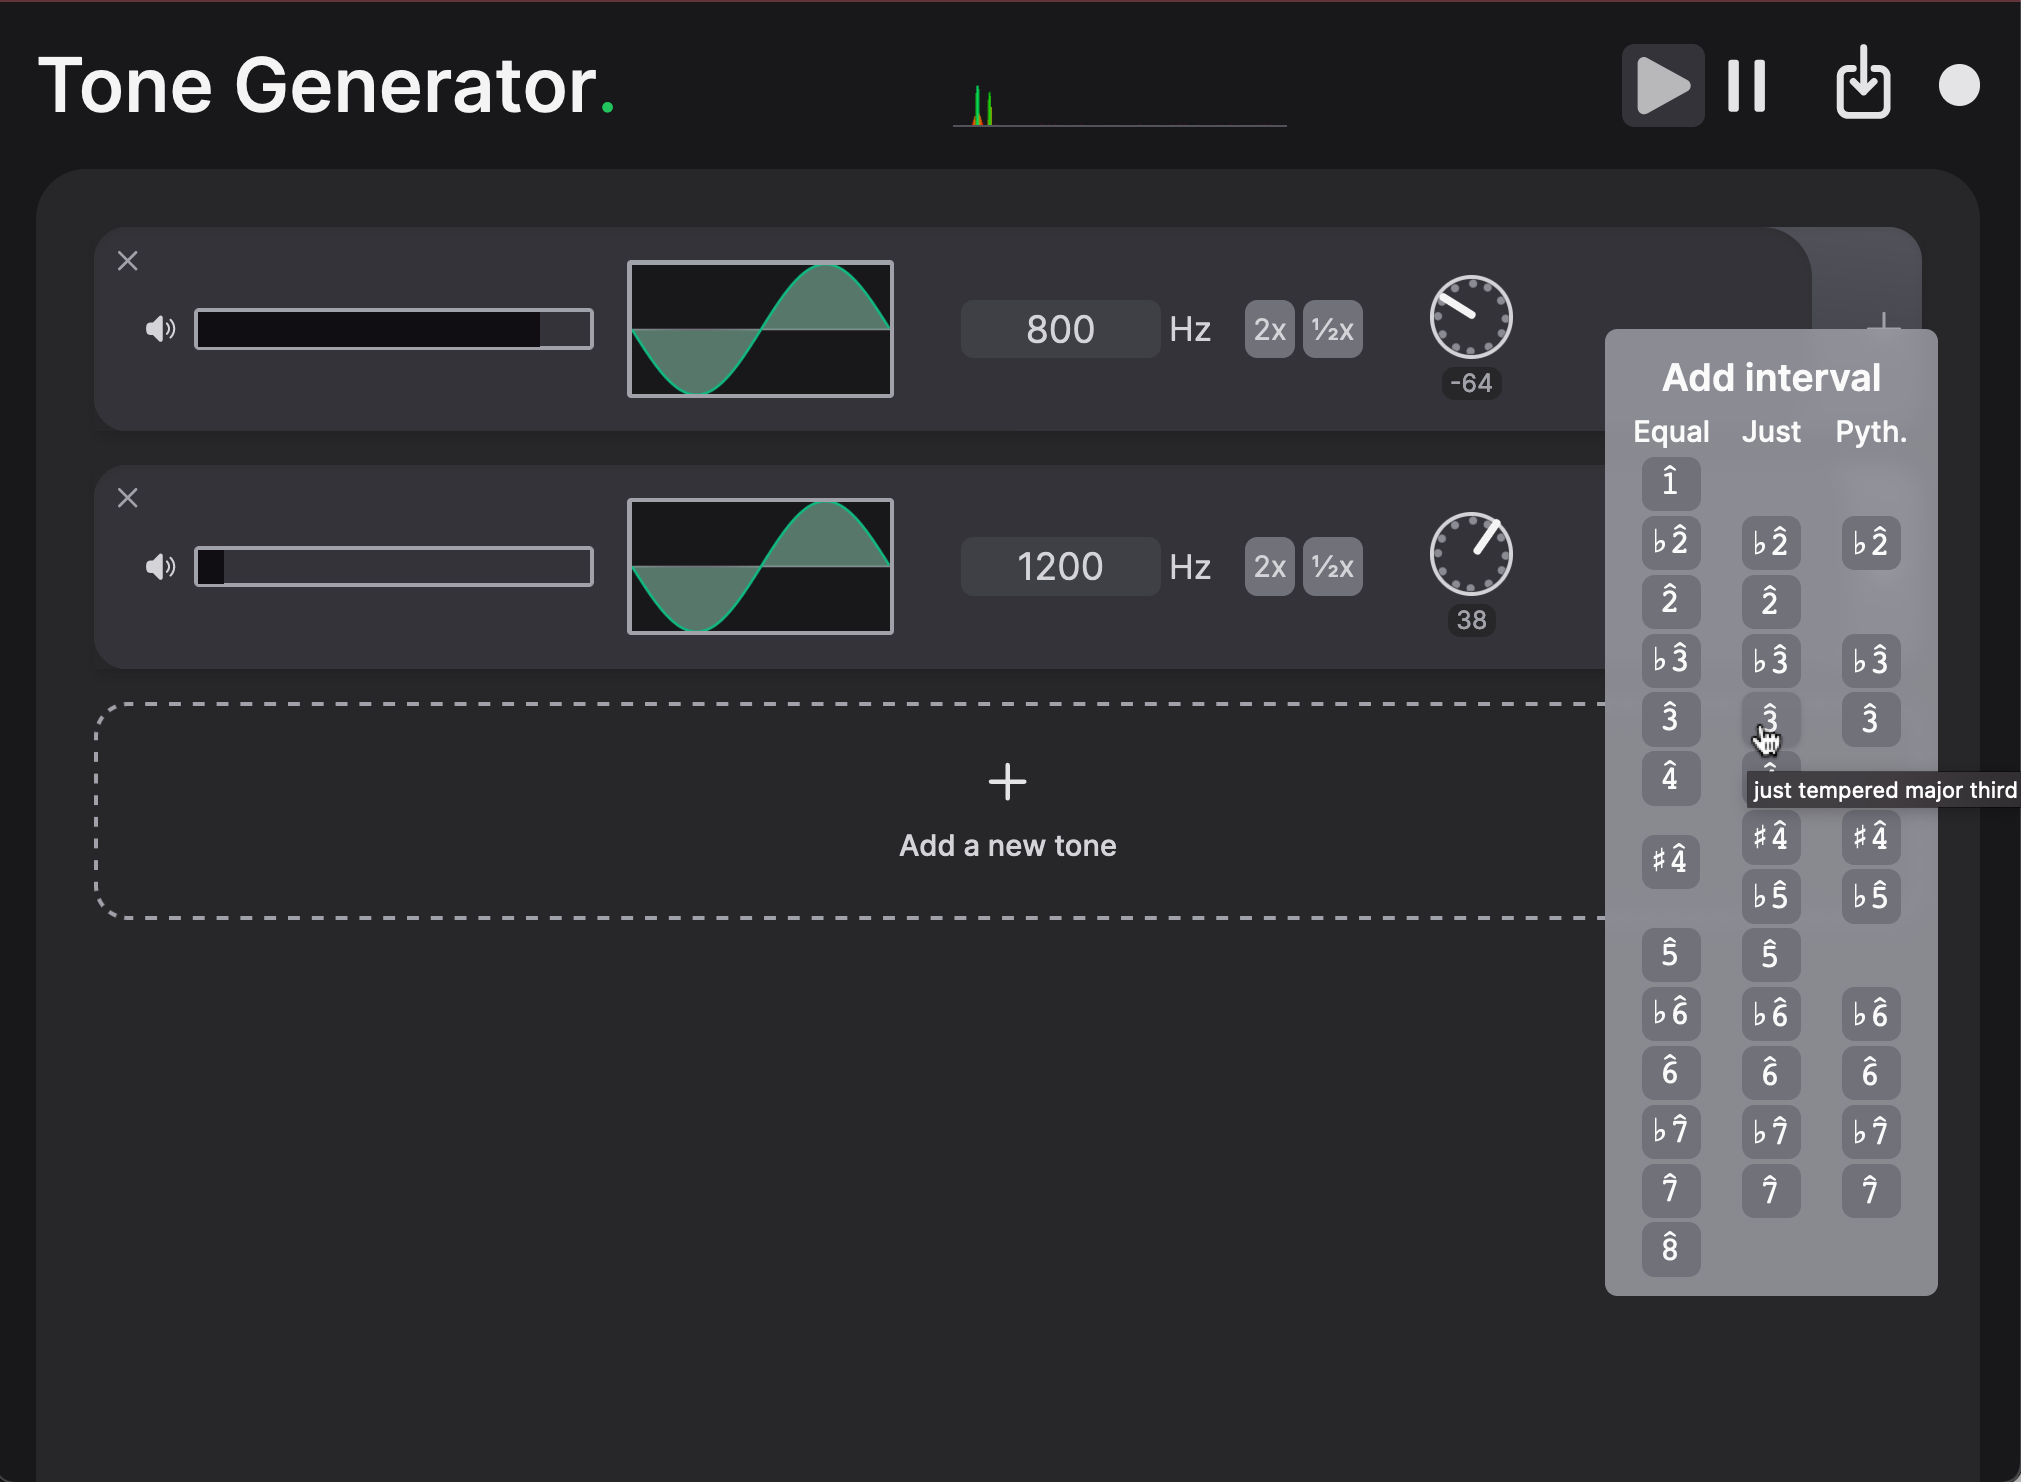
\includegraphics[width=0.85\linewidth]{tone gen ui}
\caption{The Web Interface of my Tone Generator Showing the Just- and Pythagorean-Tuned Interval Capabilities}
\label{fig:ui}
\end{figure}



\section{Experimenting as a Performer}

\subsection{"Futile Devices" And My Foray into  Harp (AOI 1)}

In AOI 1, I chose to experiment with the song “Futile Devices” by Sufjan Stevens in the global context. This song is notable for its appearance in Call Me By Your Name, a 2017 movie exploring LGBTQ issues, serving as a form of political expression. With this, I chose to experiment with the Harp, an instrument with which I had absolutely no prior experience. I arranged, transposed and improvised on the main ostinato of the song, learning about the intricacies of the Harp to make this process more simple. I first familiarized myself with basic technique and the arrangement of the Harp’s pedals. From its tuning in $C$ with all pedals in the middle position, I tuned it to $C$ dorian by flattening the $3$rd and $7$th scale degrees. This was to make my life easier, transposing the harmony from $F\sharp$ dorian/$C\sharp m$ to $C$ dorian/$Gm$ so I could use the red and black strings to better orient myself (1 and 4 respectively). I began by playing the main arpeggio, outlining a $Cm7$/G, then transitioning to the $F7sus4$ and $F7$, using both hands to get it to tempo. In variation form, I progressively added more layers to the melody, eventually incorporating it in octaves in both hands. The last portion was the most challenging, where I played the second ostinato, outlining more chord extensions, in the RH, while maintaining both the first ostinato and the harmony in the LH. Overall, I was proud of my progress in about a week in-class and without any instruction.


\subsection{Improvising on Coltrane's "Alabama" Vamp (AOI 1)}

In AOI 1, I am choosing to experiment with John Coltrane’s “Alabama,” in the local context. This song is AOI 1, because Coltrane intended it to reflect the state of the civil rights movement in the US. It’s said that he attempted to mimic the cadences of Martin Luther King Junior’s speeches with his improvisational melody. I plan to experiment with the idea of sitting on a single harmony with improvisation in the melody. In Coltrane’s work, he sits on this C minor harmony, with a melodic emphasis on a $\flat7–1$ resolution, or a $v–i$ resolution. I will experiment with a $Fm–F$ dorian harmony in an improvisational way, focusing on the sound of a $iv–i$ resolution, to create a similar tone to Coltrane in a novel way.

\subsection{Reharmonizing a National Anthem (AOI 1)}

In AOI 1, I chose to experiment with the Russian Anthem, in the global context. I planned to experiment with the harmony of the piece—specifically by reharmonizing elements of it and varying the key. I planned to do this because it employs a simple harmony with virtually no chord extensions or modulations. By experimenting with it, I will convert it towards a more jazz-influenced style, with a more complicated harmony, including a number of distant modulations scattered throughout. In this way, I plan to transform the melody into a different context, enriching its simplicity with new harmony. 

\begin{figure}[H]
\centering
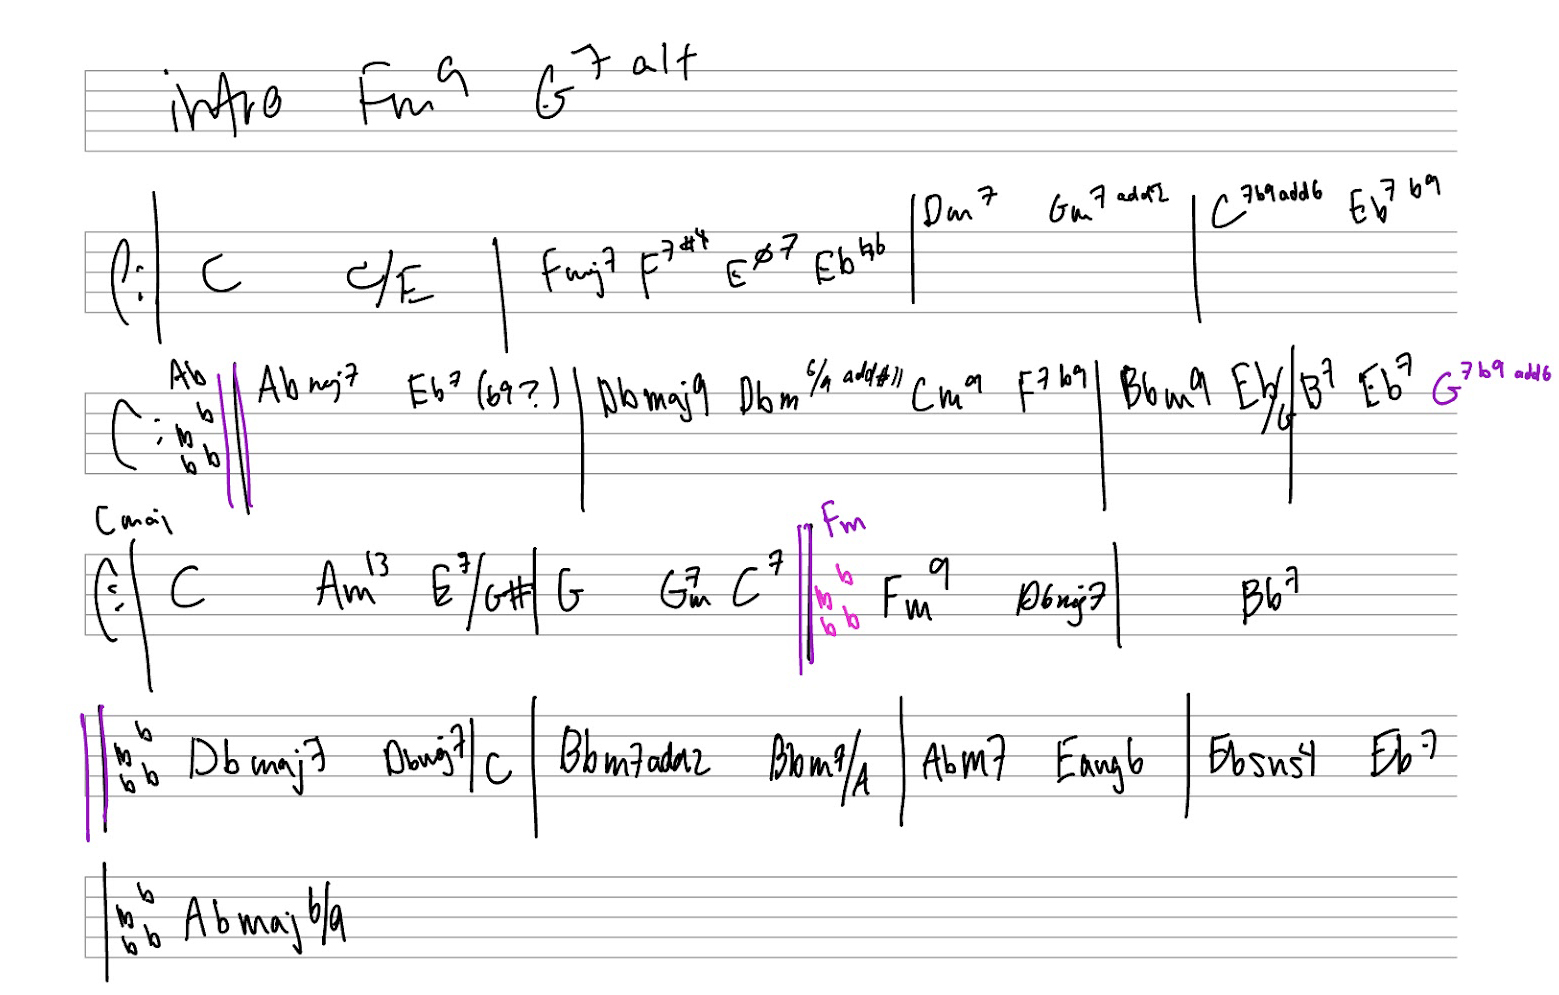
\includegraphics[width=0.85\linewidth]{anthem}
\caption{My Handwritten Lead Sheet for the Russian Anthem Reharm}
\label{fig:anthem}
\end{figure}


\section{Track List}

\begin{table}[H]
\centering
\begin{tabularx}{0.9\textwidth}{@{}lX@{}X@{}}
\toprule
\textbf{Track} & \textbf{Start} & \textbf{End} \\ \midrule
"The Falling Mysts" EDM for Chamber Orchestra & 0:00 & 2:15 \\
5/8 Time Signature Etude for Piano and Drums & 2:19 & 3:47 \\
Pure Sine Waves and Just Intonation & 3:51 & 4:40 \\ \bottomrule
\end{tabularx}
\caption{Experimenting as a Creator}
\vspace*{0.5cm}
\begin{tabularx}{0.9\textwidth}{@{}lX@{}X@{}}
\toprule
\textbf{Track} & \textbf{Start} & \textbf{End} \\ \midrule
Arranging for and Learning the Harp & 4:44 & 6:14 \\
Coltrane's "Alabama" and Modal Improvisation\hspace*{10pt} & 6:18 & 8:16 \\
Reharmonizing a National Anthem & 8:20 & 9:38 \\ \bottomrule
\end{tabularx}
\caption{Experimenting as a Performer}
\end{table}

\iffalse
\pagebreak

\begin{figure}[H]
\centering
\begin{tabular}{cc}
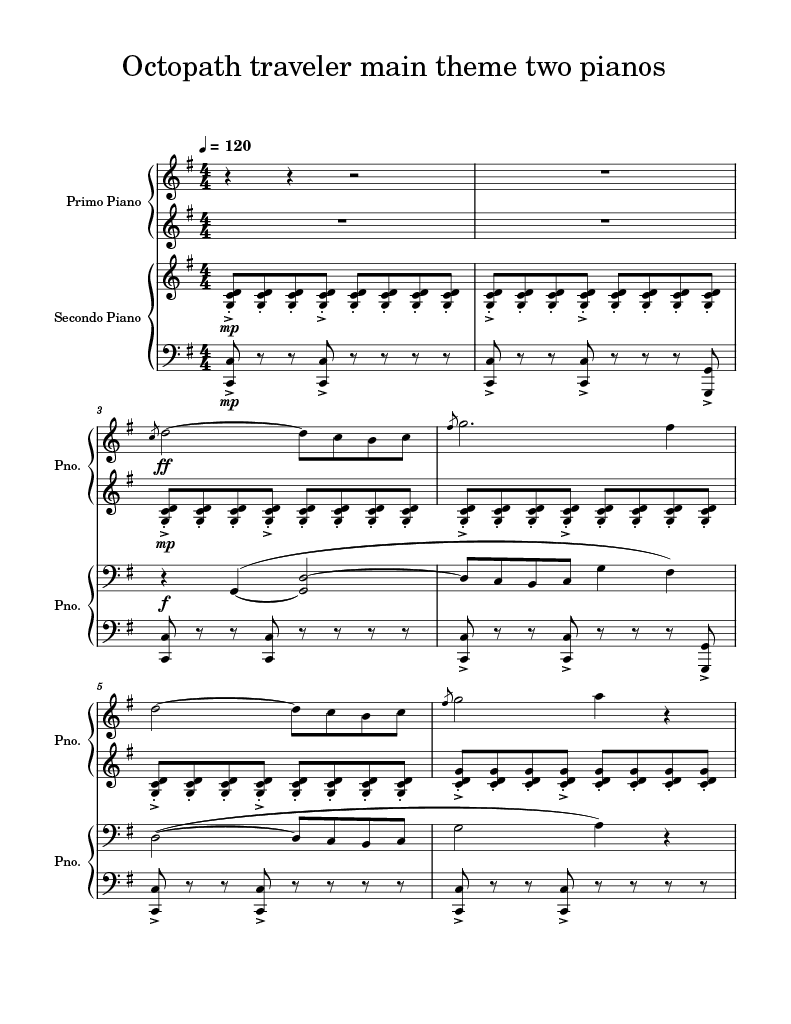
\includegraphics[width=.4\linewidth, trim=30 100 30 20, clip]{octopathscore/octopathscore1024_1.png} &
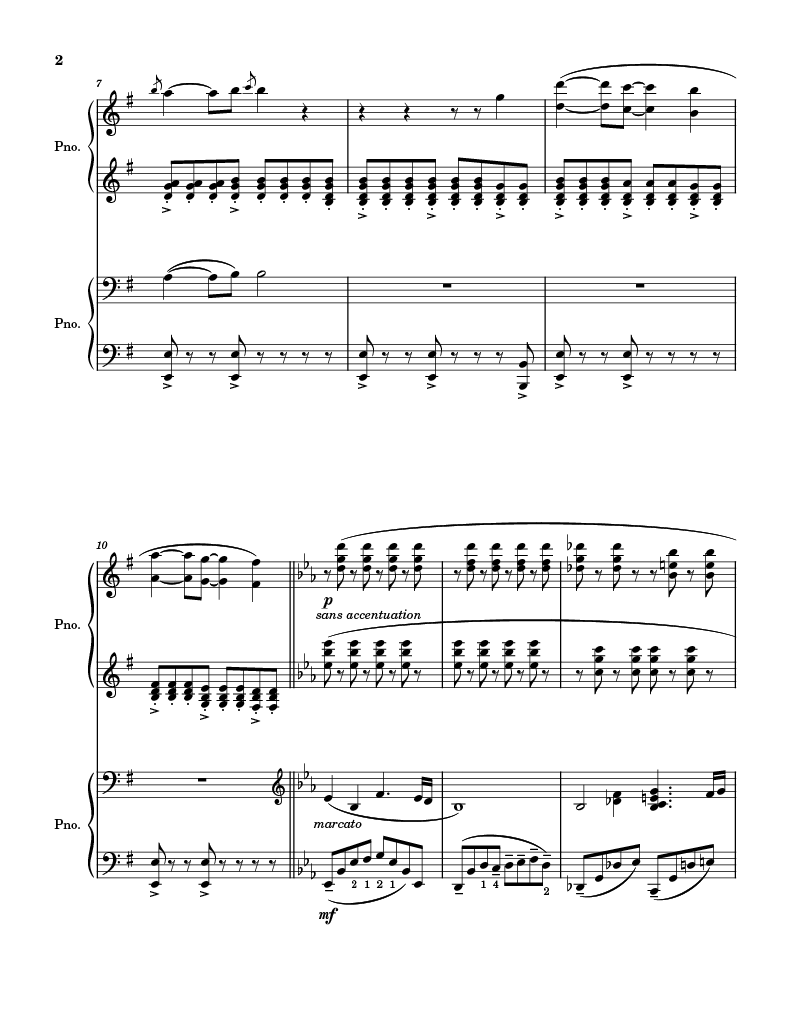
\includegraphics[width=0.4\linewidth, trim=30 100 30 20, clip]{octopathscore/octopathscore1024_2.png} \\
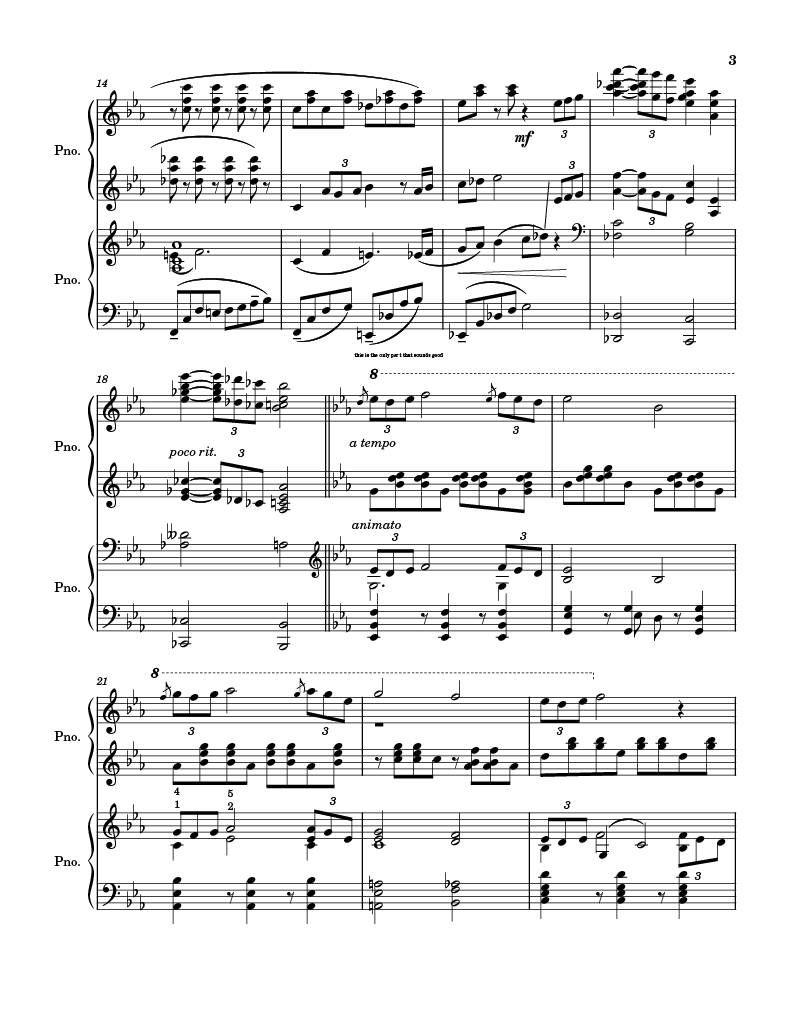
\includegraphics[width=0.4\linewidth, trim=30 100 30 20, clip]{octopathscore/octopathscore1024_3.png} &
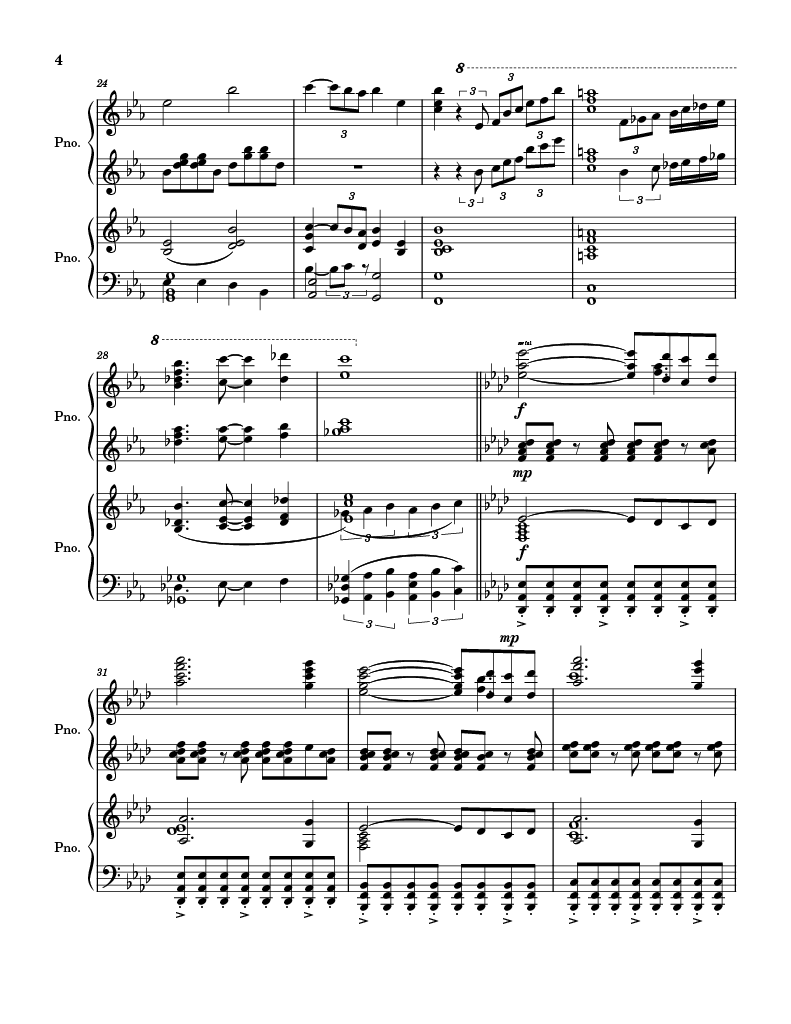
\includegraphics[width=0.4\linewidth, trim=30 100 30 20, clip]{octopathscore/octopathscore1024_4.png}
\end{tabular}
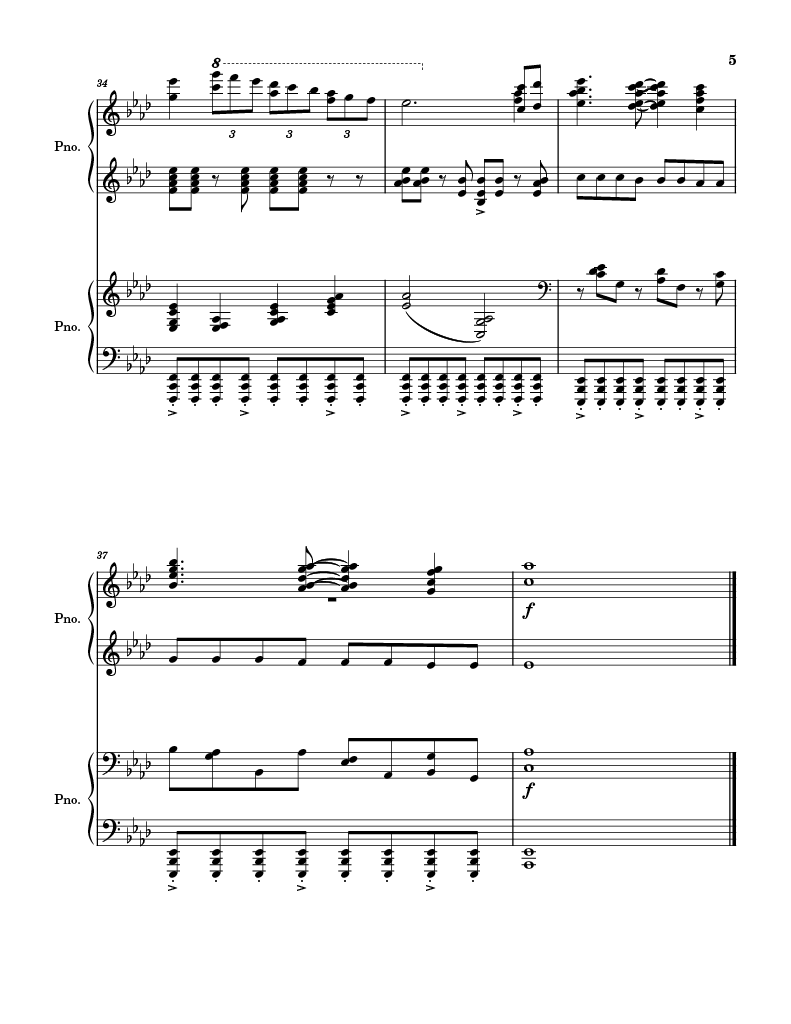
\includegraphics[width=0.4\linewidth, trim=30 100 30 20, clip]{octopathscore/octopathscore1024_5.png}
\caption{My Arrangement Score for Exploring as a Creator}
\end{figure}
\fi

\section{References}
\printbibliography[heading=none]

\section{Appendix}
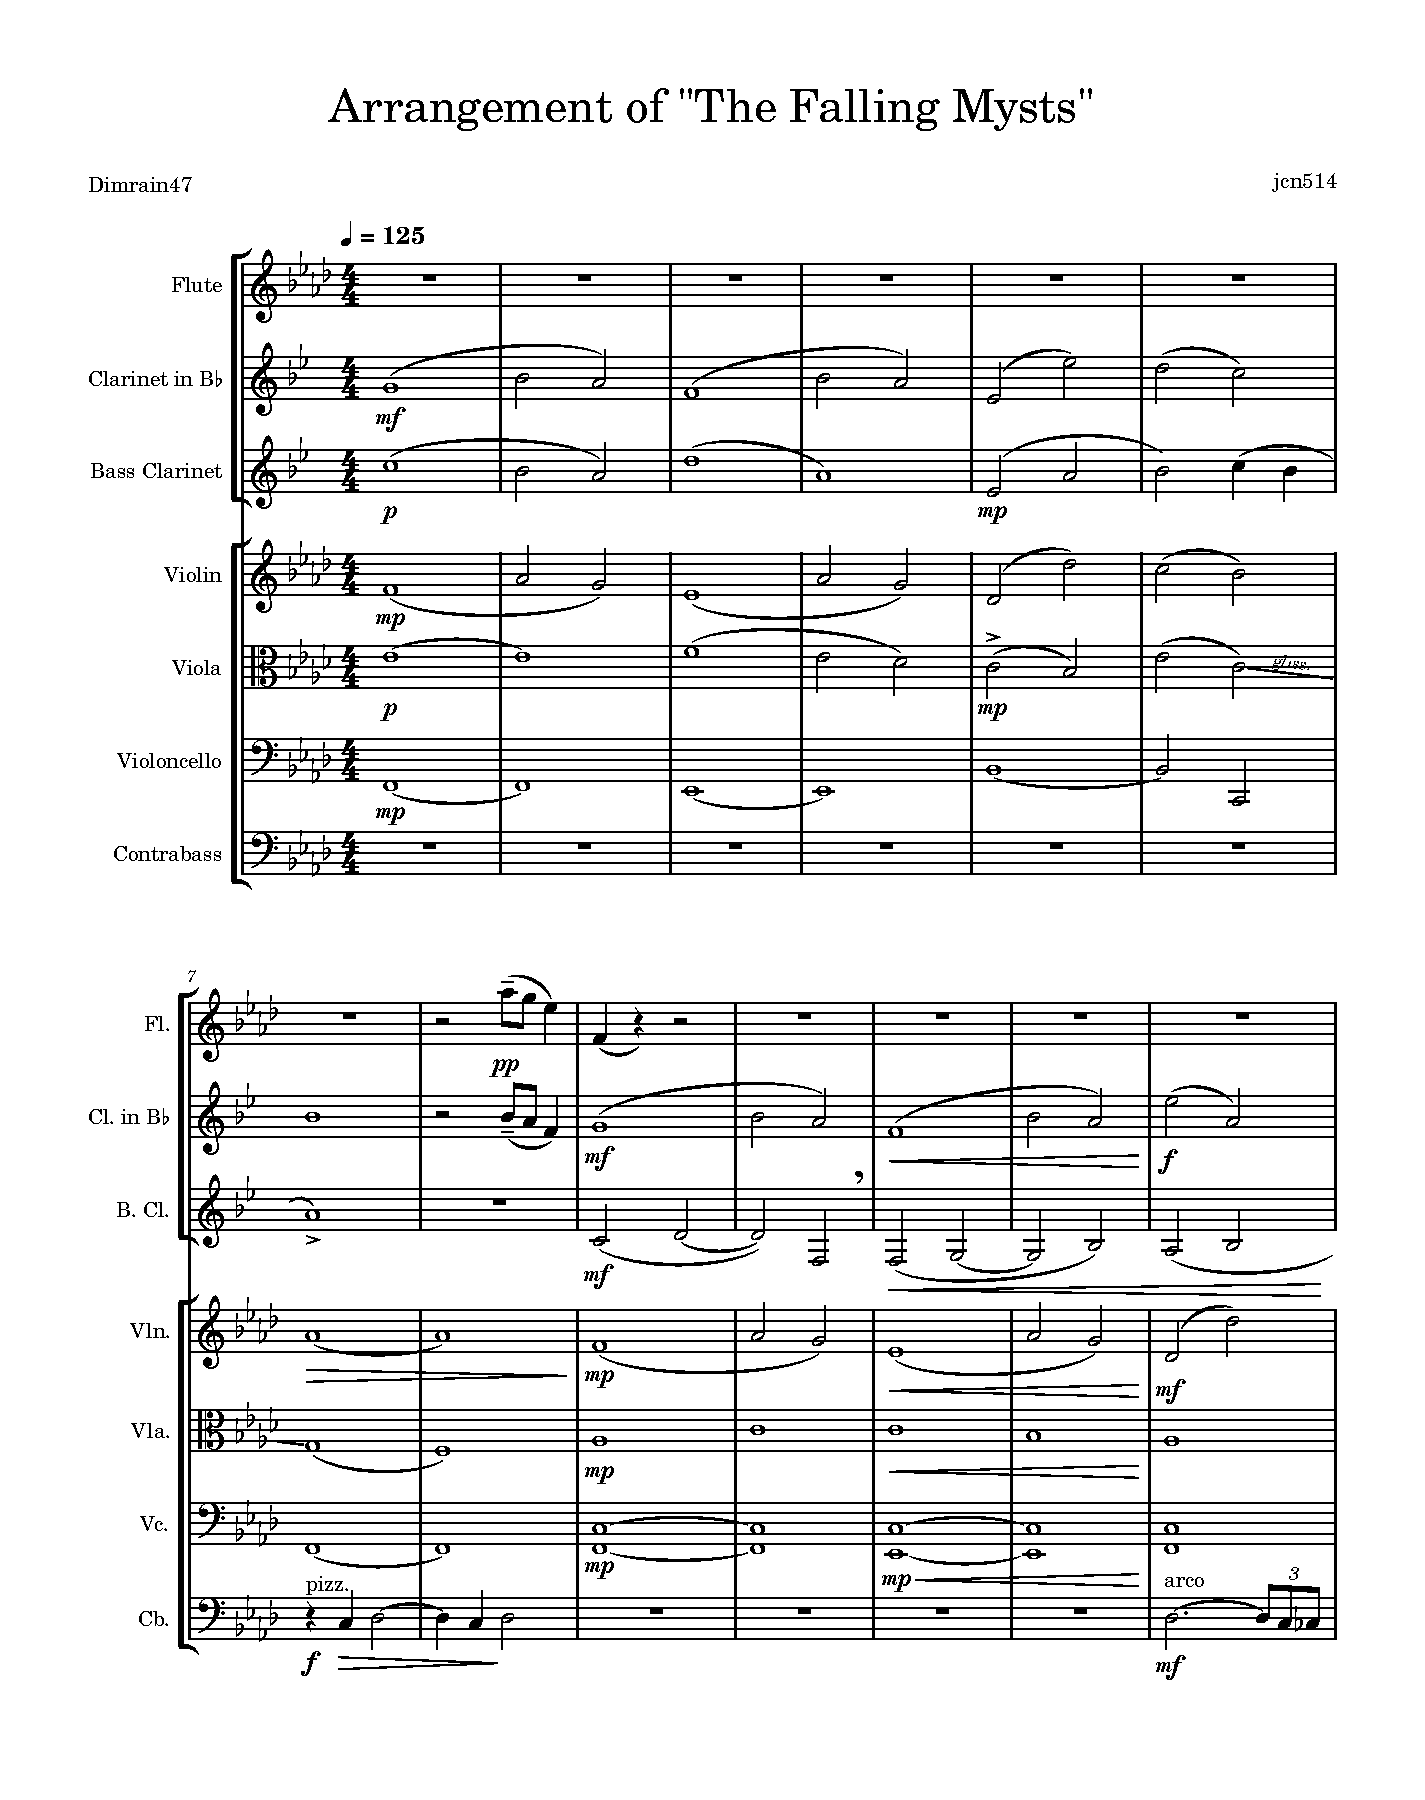
\includepdf[pages=-]{fallingmysts.pdf}

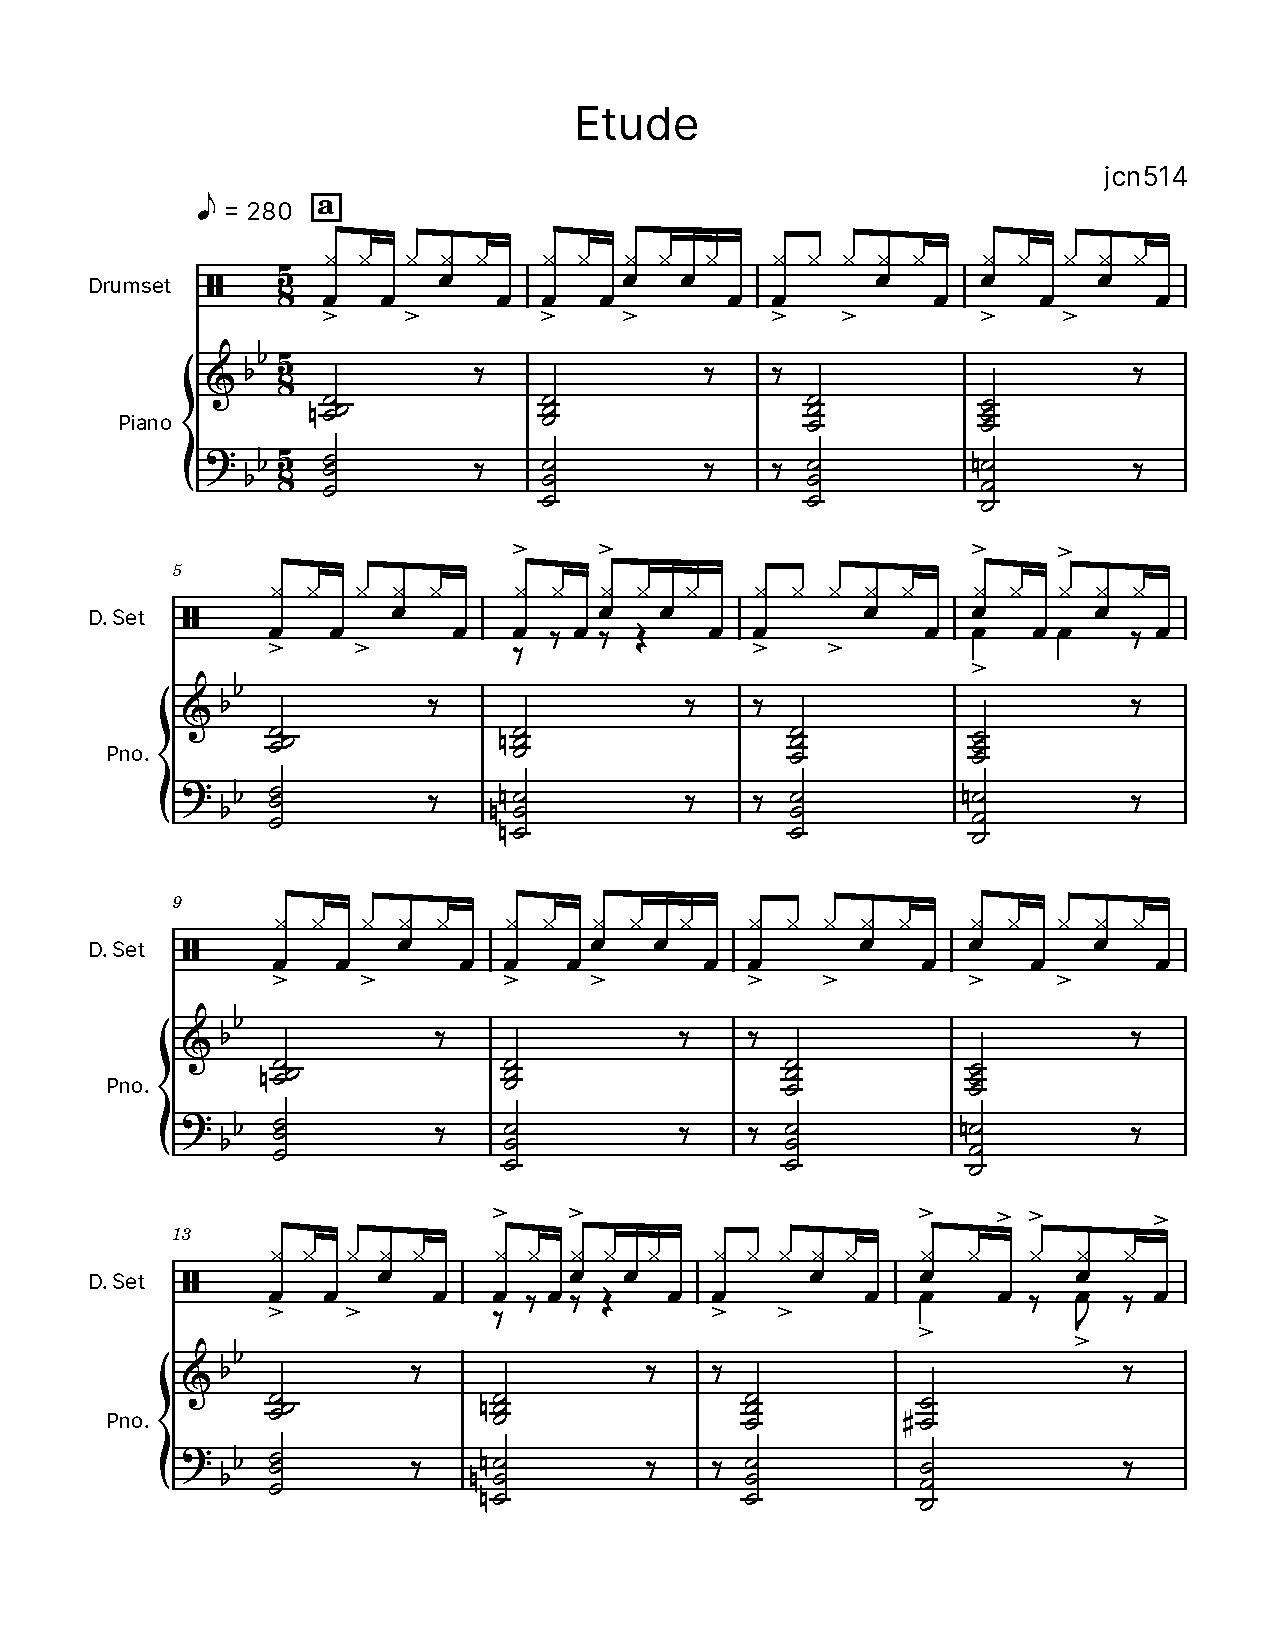
\includepdf[pages=-]{5o8.pdf}


\end{document}